% !TeX root = ../sustechthesis-example.tex

\chapter{补充内容}

% 一些数学、图片、表格、代码等的补充... 
% \begin{figure}
%     \centering
%     \caption[RTMQ测控板实物图]{RTMQ测控板实物图\label{fig:rtmq_board_real}}
%     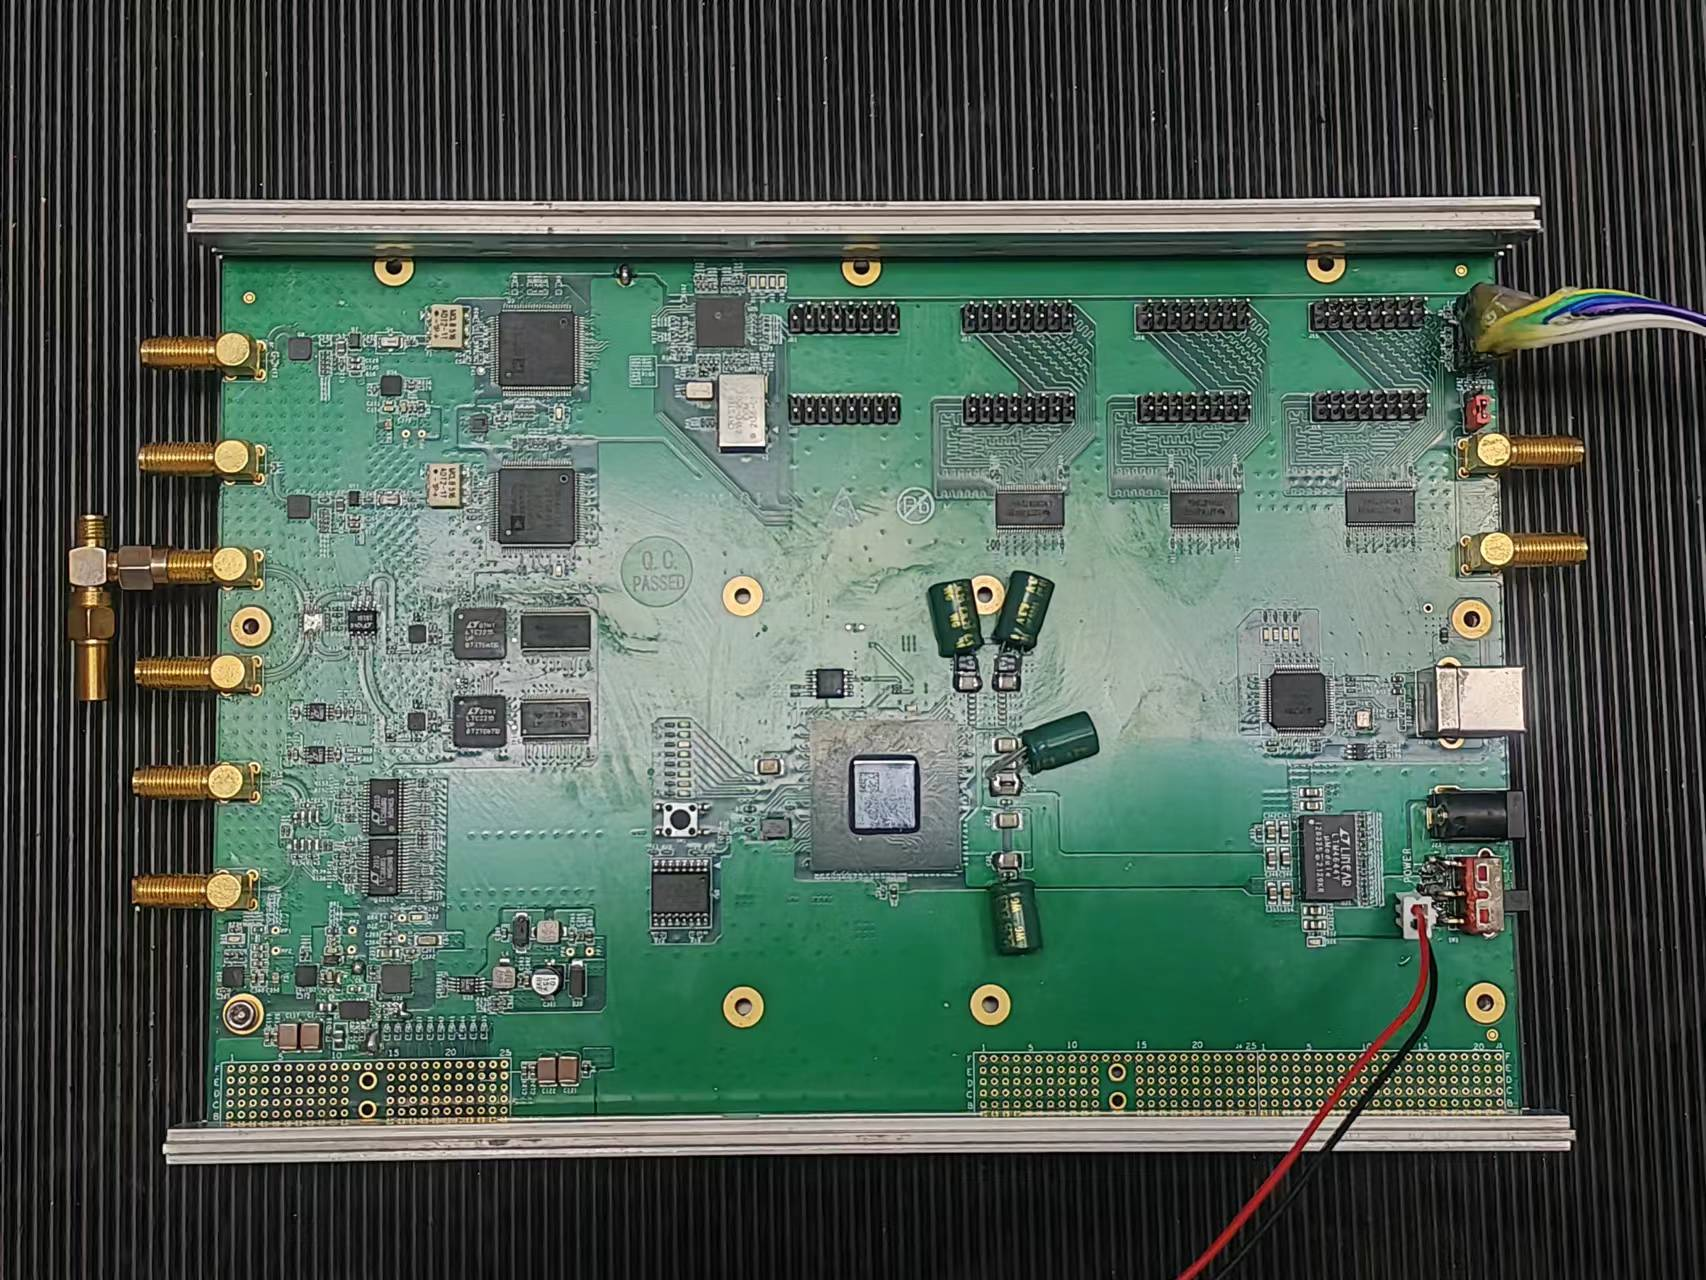
\includegraphics[width=1.0\linewidth]{rtmq/rtmq_board_real}
% \end{figure}

% \begin{figure}
%     \centering
%     \caption[8位超前进位加法器的FPGA实现结构图]{8位超前进位加法器的FPGA实现结构图(Vivado)\label{fig:ahead_adder_8bits}}
%     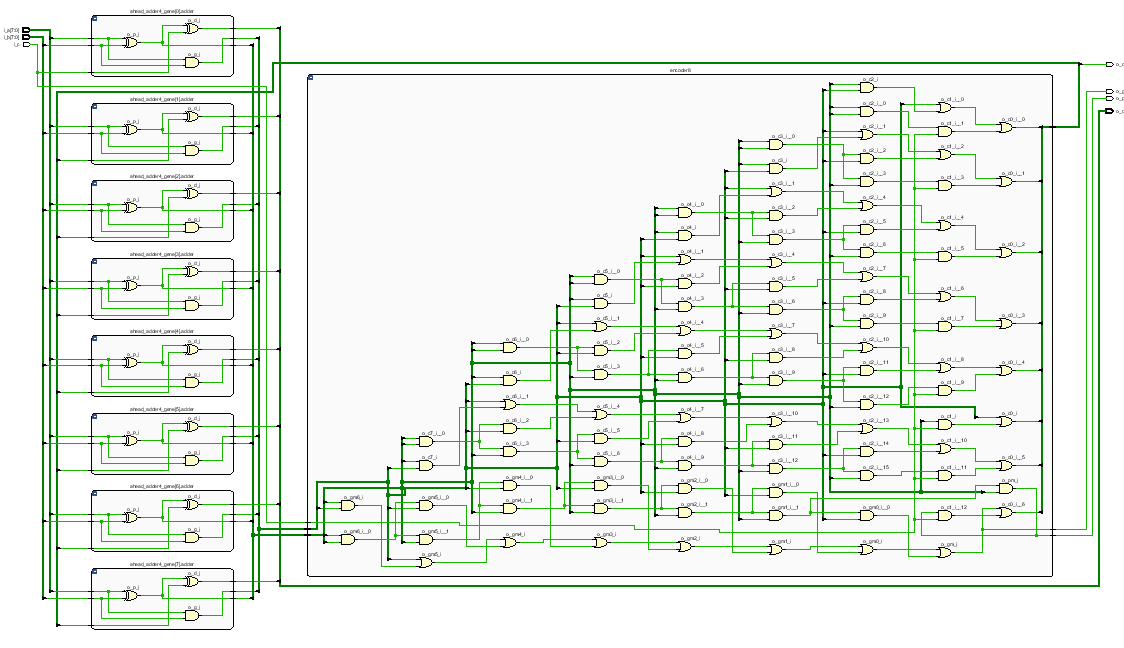
\includegraphics[width=1.0\linewidth]{rtmq/ahead_adder_8bits}
% \end{figure}

\begin{figure}
    \centering
    \caption[16位超前进位加法器的FPGA实现结构图]{16位超前进位加法器的FPGA实现结构图(Vivado)\label{fig:ahead_adder_16bits}}
    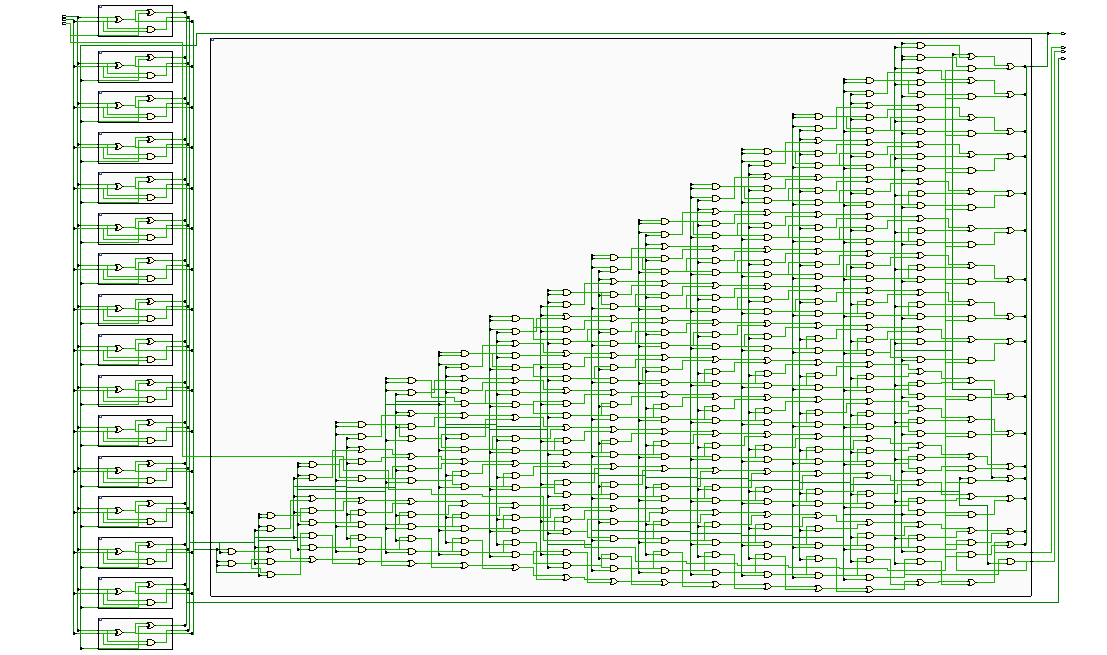
\includegraphics[width=1.0\linewidth]{rtmq/ahead_adder_16bits}
\end{figure}


\begin{figure}
    \centering
    \caption[32位Booth乘法器编码和加法树表]{32位Booth乘法器编码和加法树表\label{fig:booth_multiplier_32bits_basic}}
    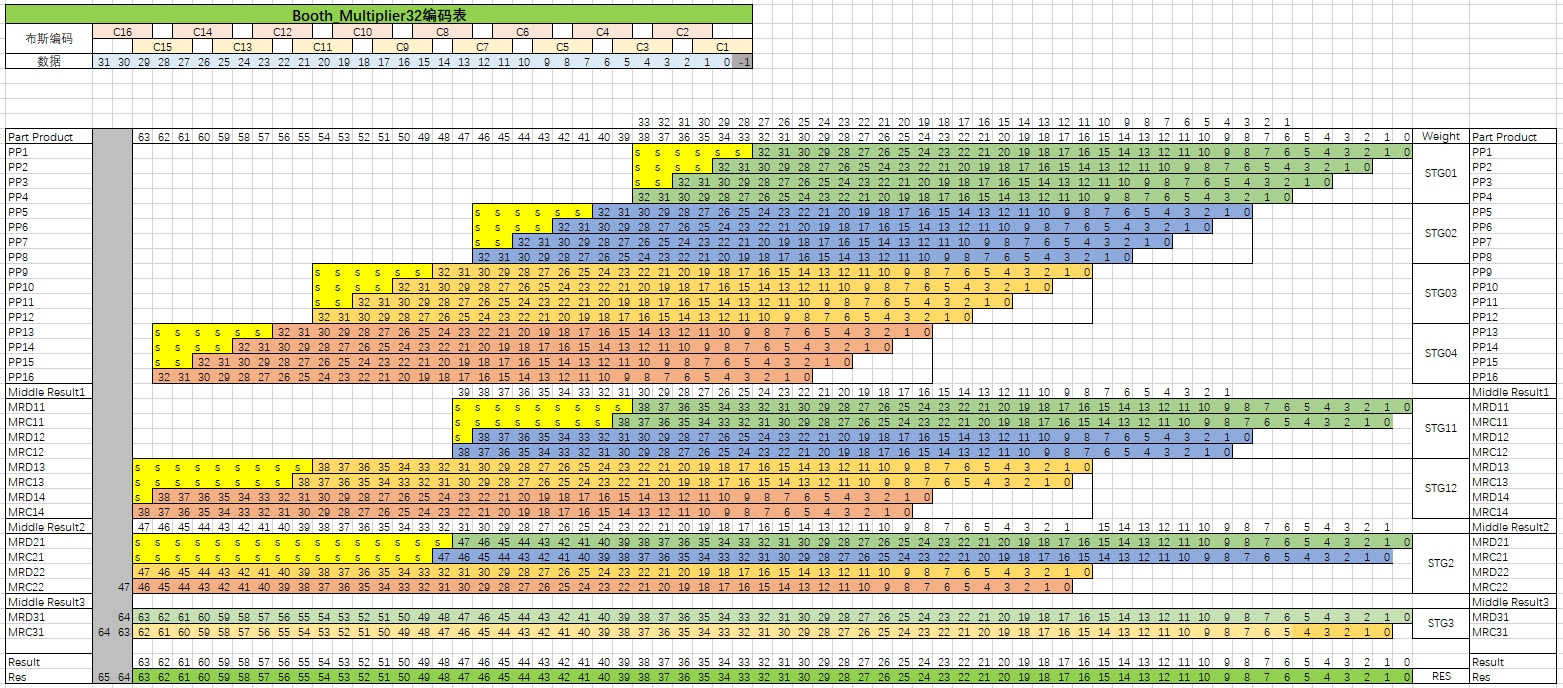
\includegraphics[width=1.0\linewidth]{rtmq/booth_multiplier_32bits_basic}
\end{figure}

% \begin{figure}
%     \centering
%     \caption[脉冲激光拍频锁定系统图]{脉冲激光拍频锁定系统图\label{fig:beat_note_stabilization_real}}
%     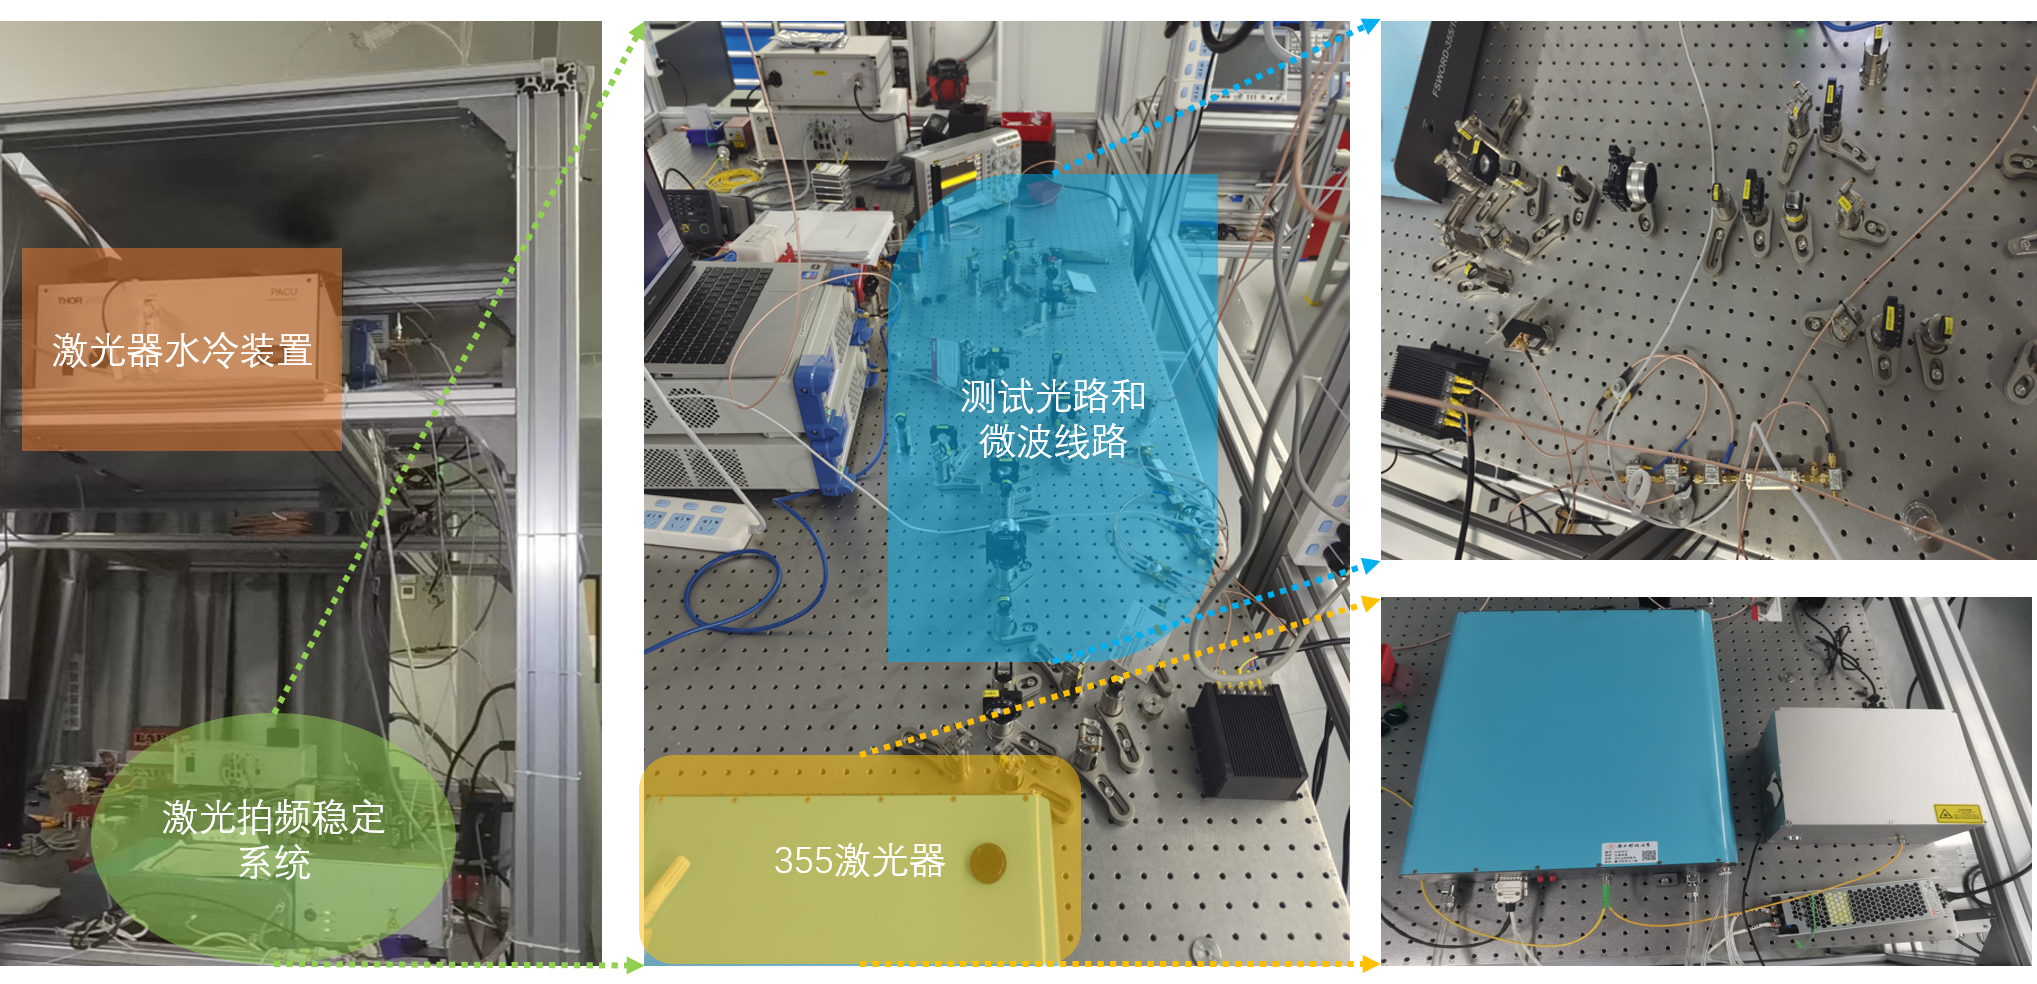
\includegraphics[width=1.0\linewidth]{beat_note_stabilization_real}
% \end{figure}

\begin{figure}
    \centering
    \caption[阱频锁定模块实验测试图]{阱频锁定模块实验测试图\label{fig:trap_frequency_lock_real}}
    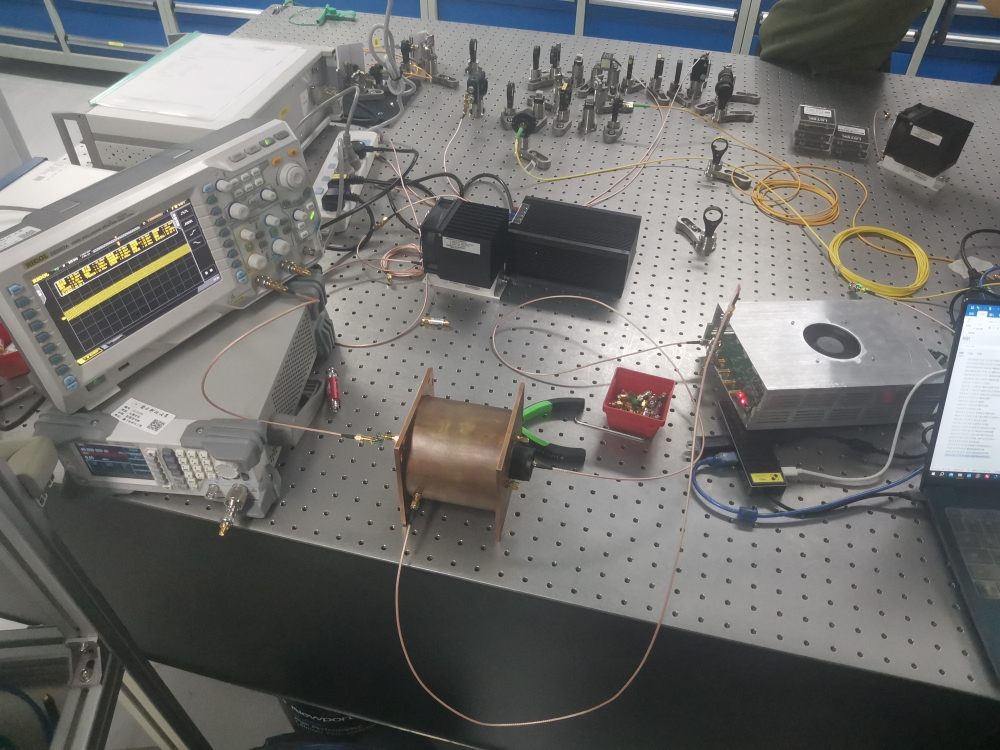
\includegraphics[width=1.0\linewidth]{trap_frequency_lock_real}
\end{figure}

% \begin{figure}
%     \centering
%     \caption[激光功率锁定系统测试图]{激光功率锁定系统测试图\label{fig:laser_stabilization_real}}
%     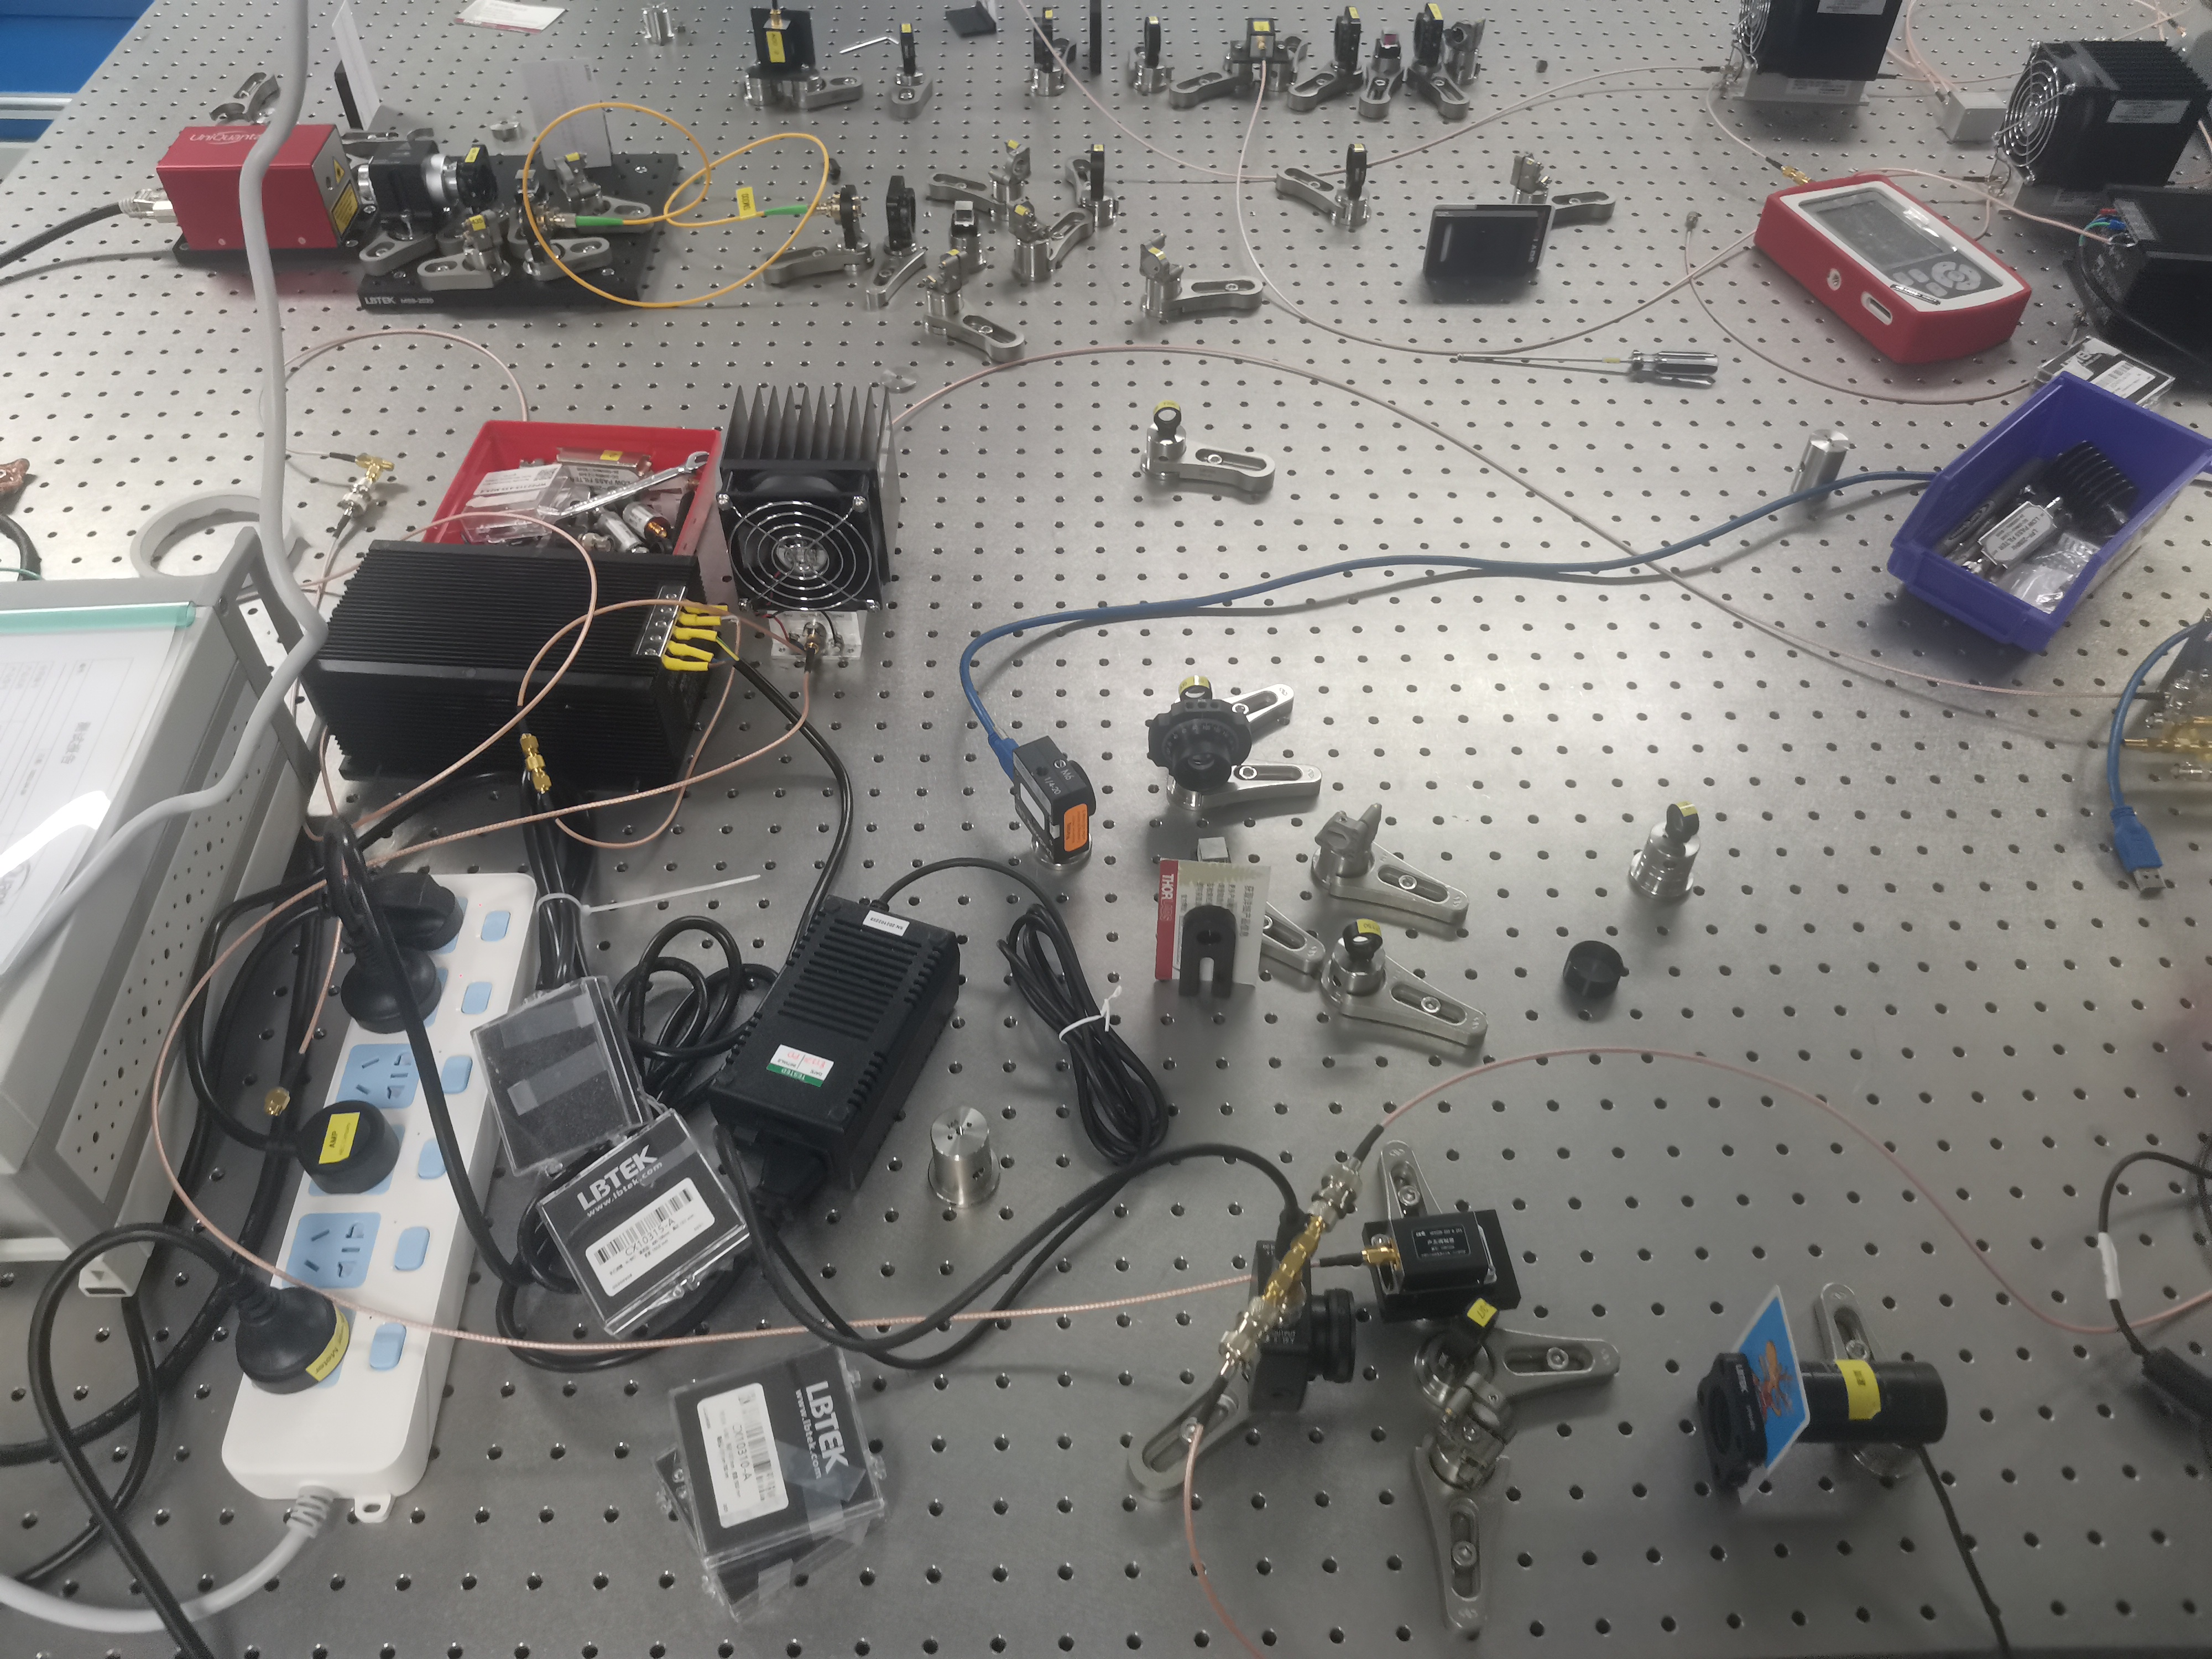
\includegraphics[width=1.0\linewidth]{laser_stabilization_real}
% \end{figure}

\begin{figure}
    \centering
    \caption[激光功率外部稳定的拓展方案架构图]{激光功率外部稳定的拓展方案架构图\label{fig:laser_stabilization}}
    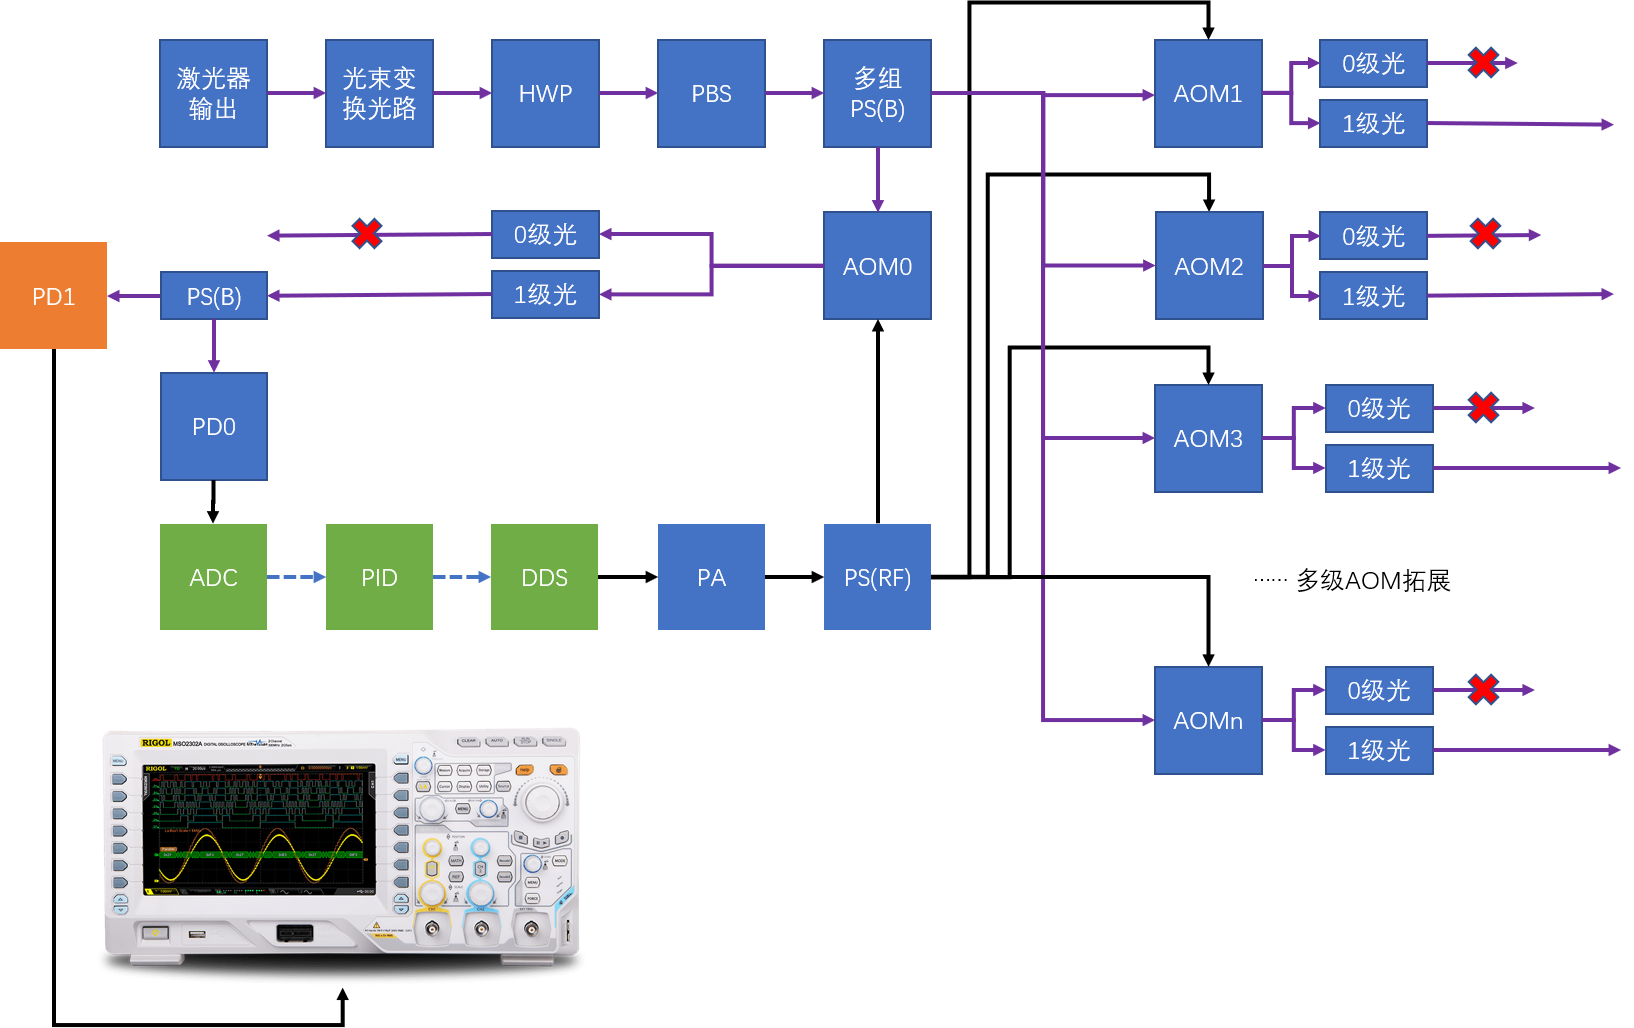
\includegraphics[width=1.0\linewidth]{laser_stabilization1}
\end{figure}

\begin{figure}
    \centering
    \caption[实验室中实际离子阱系统图]{实验室中实际离子阱系统图\label{fig:ion_trap_system}}
    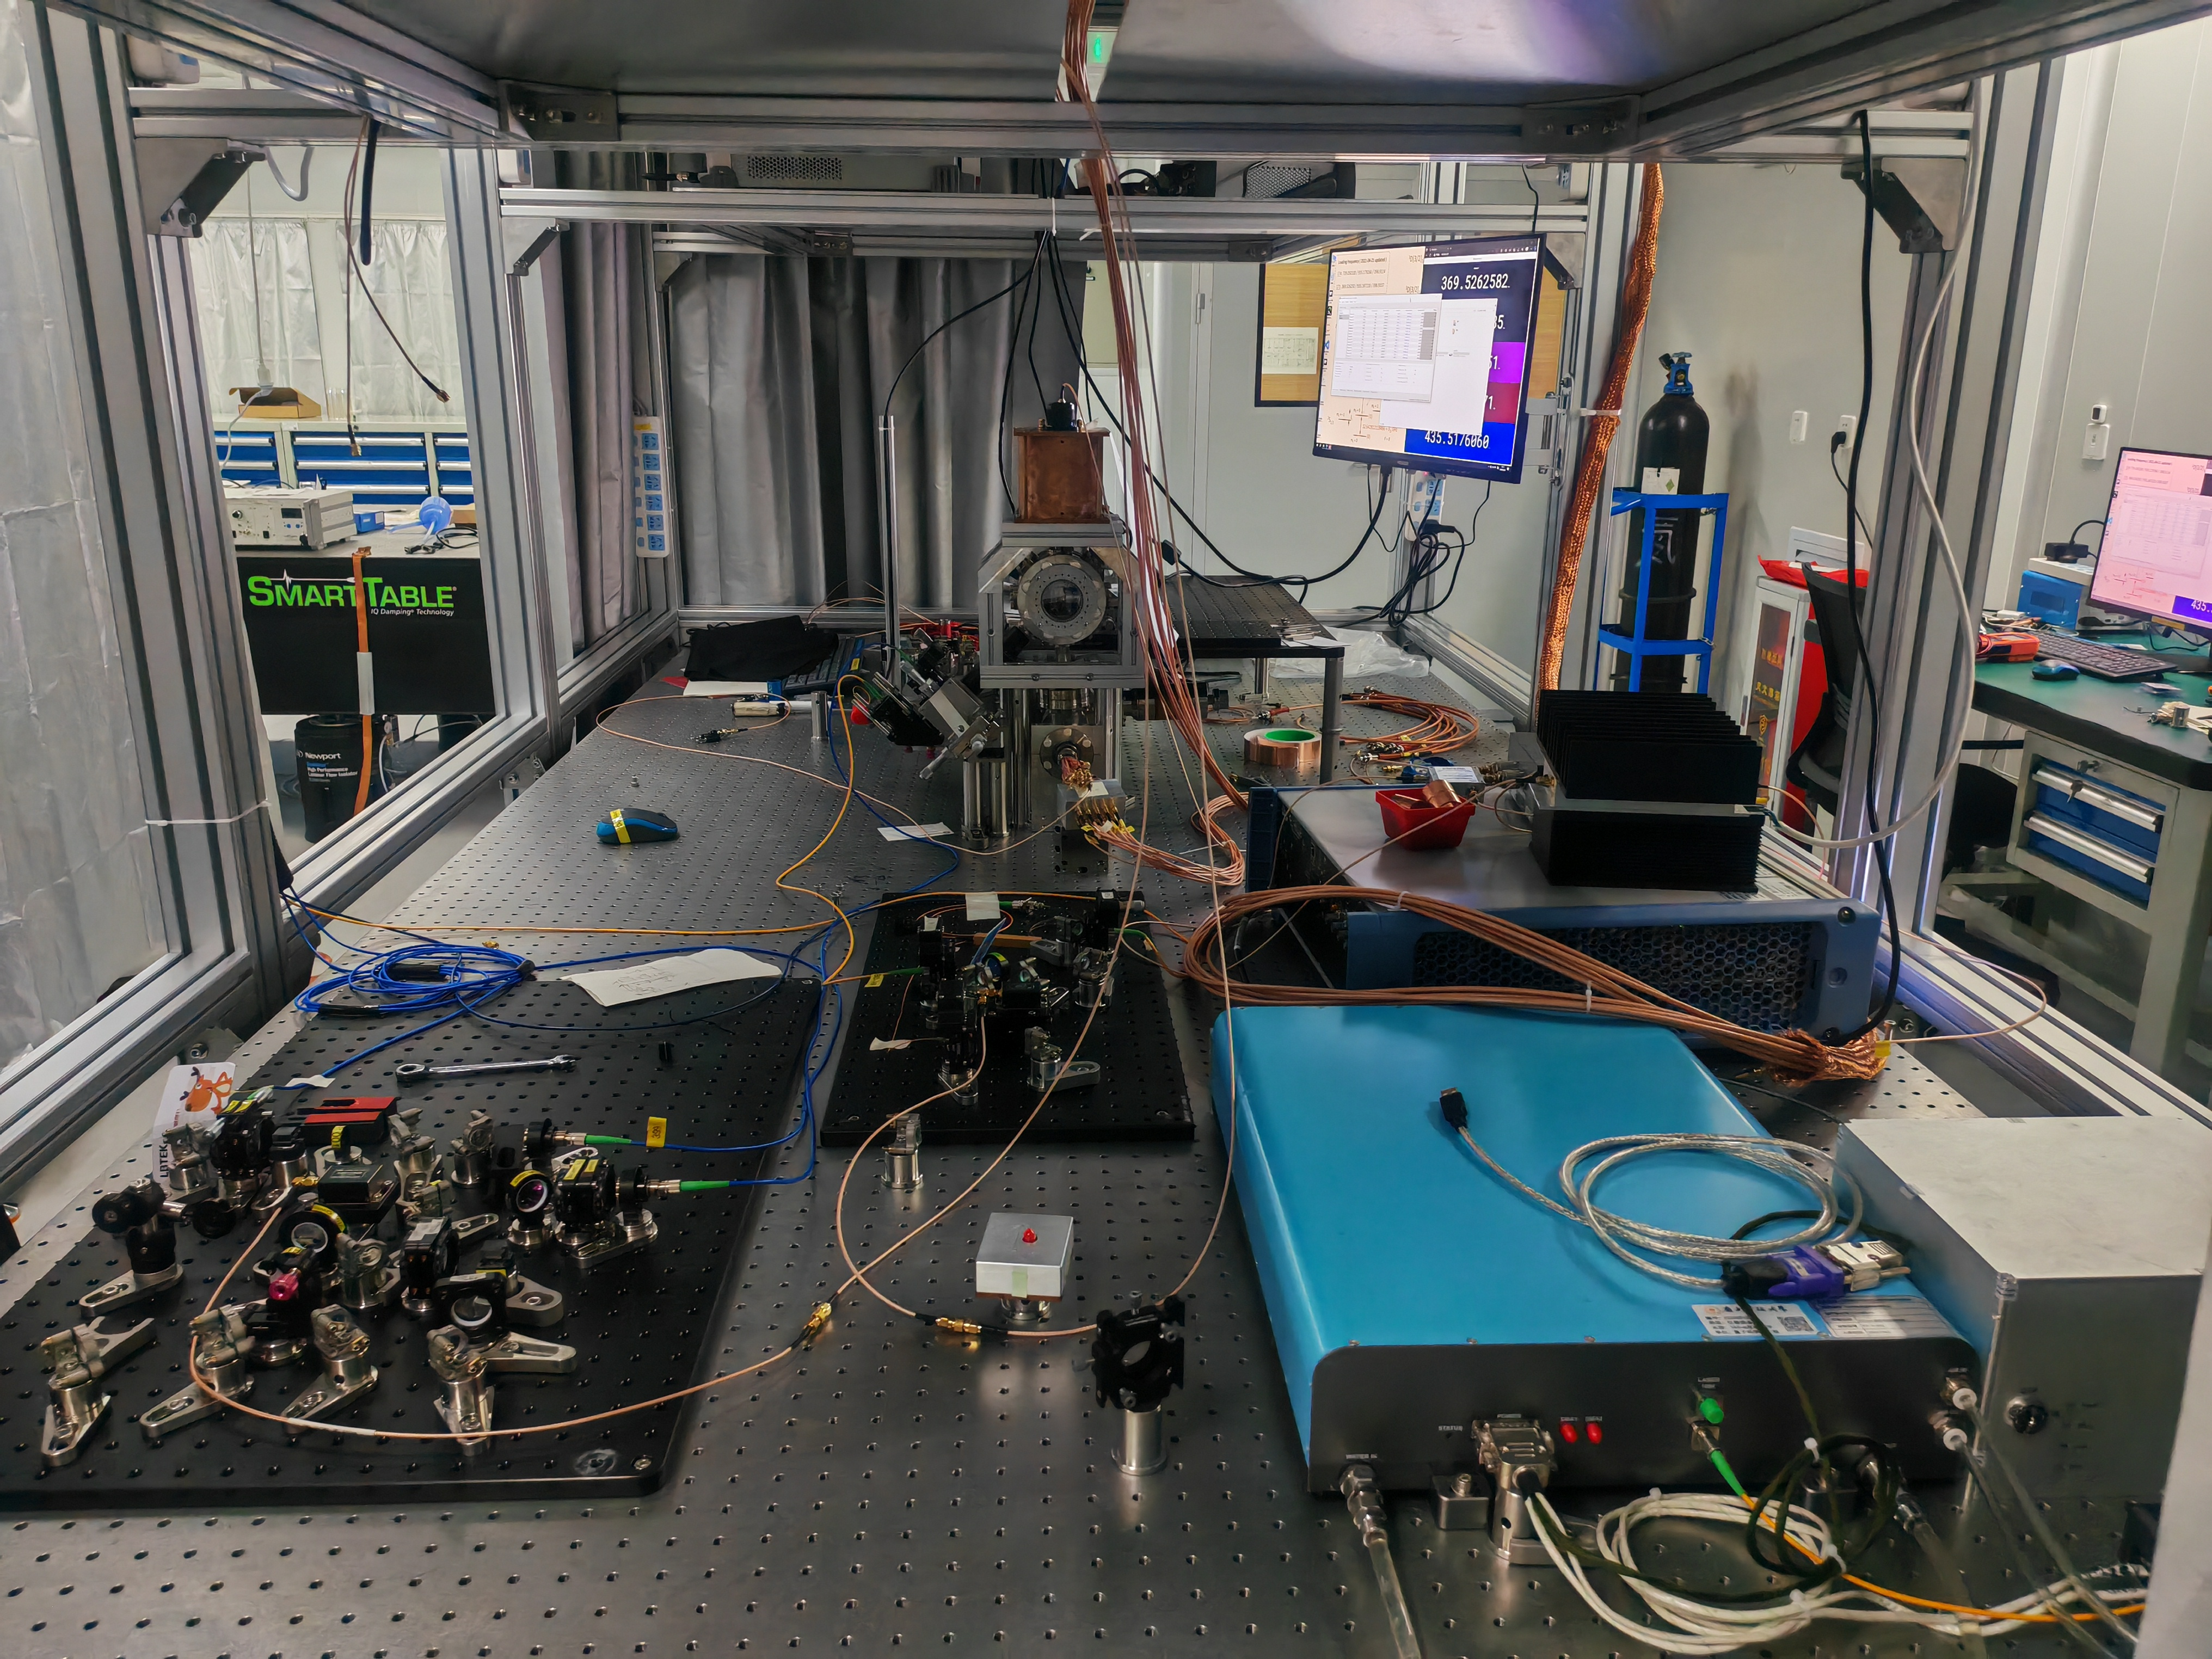
\includegraphics[width=1.0\linewidth]{ion_trap_system}
\end{figure}